% This is a borrowed LaTeX template file for lecture notes for CS267,
% Applications of Parallel Computing, UCBerkeley EECS Department.

% To familiarize yourself with this template, the body contains
% some examples of its use.  Look them over.

\documentclass[a4paper]{article}

%
% ADD PACKAGES here:
%

\usepackage{amsmath,amsfonts,graphicx,multicol}
\usepackage[margin=1in]{geometry}
\usepackage{amsthm}
\usepackage{amsmath}

\setlength{\parskip}{\baselineskip} % Set space between paras
\setlength{\parindent}{0pt} % No para indentation

\newtheorem{theorem}{Theorem}[section]
\newtheorem{corollary}[theorem]{Corollary}
\newtheorem{lemma}[theorem]{Lemma}
\newtheorem{definition}[theorem]{Definition}
\newtheorem{remark}[theorem]{Remark}

\begin{document}

%% Header

\pagestyle{myheadings}
   \thispagestyle{plain}
   \newpage
   \noindent
   \begin{center}
   \framebox
   {
      \vbox{\vspace{2mm}
        \hbox to 6.28in { {\bf CSE-483: Mobile Robotics
	    \hfill Monsoon 2019} }
      \vspace{4mm}
        \hbox to 6.28in { {\Large \hfill Camera calibration (DLT, Zhang's)  \hfill} } %% Fill here
        \vspace{2mm}
        \hbox to 6.28in { {\it Prepared by: Udit Singh Parihar, Sai Shubodh P \hfill} } %% Fill here
        \vspace{2mm}}
   }
   \end{center}
   \markboth{Camera Calibration}{Camera Calibration} %% Fill here


% Your note begins here...

In this note, we discuss how to obtain the intrinsic and extrinsic calibration parameters of a camera given the coordinates of object points $\vec{X}$ and the observed coordinates of those object points in the image $\vec{x}$. There are two methods to do this:

\begin{enumerate}
    \item Direct Linear Transform: This method maps any object point $\vec{X}$ to the image point $\vec{x}$ and assumes that we do not know anything about the intrinsic nor extrinsic parameters. Here, the object points should be non-planar in the 3 dimensional world. In this method, we will be needing at least 6 pairs of points to extract the parameters.
    \item Zhang's method: This also assumes that we do not know anything about the intrinsic nor extrinsic parameters. But here, the object points are considered to lie on a 2D known structure of known size, typically a checkerboard. We leverage the fact that they lie on the same plane to make it easier to extract the world coordinates using known structures. Hence it reduces the number of minimum pairs require to obtain camera's parameters, specifically equal to 4 pairs.
\end{enumerate}

\section{Direct Linear Transform}
The pin hole camera equation: 

\begin{equation}
\vec{x}= KR [I_{3}| - X_{O}]\vec{X}
\label{eq1}
\end{equation}
\subsection{Finding combined calibration matrix, P}
We can combine the camera intrinsic and extrinsic matrices as a single matrix P:

\begin{equation}
\vec{x}= P \vec{X}
\label{eq2}
\end{equation}

Expanding x and X:
\begin{center}
\\$ \begin{bmatrix} u\\ v\\ w \end{bmatrix}   =   \begin{bmatrix}p_{11} & p_{12} & p_{13} & p_{14}\\ p_{21} & p_{22} & p_{23} & p_{24}\\ p_{31} & p_{32} & p_{33} & p_{34}\end{bmatrix} \begin{bmatrix} U\\ V\\ W\\ T \end{bmatrix} $

$ \begin{bmatrix} u/w\\ v/w\\ 1 \end{bmatrix}  = P  \begin{bmatrix} U/T\\ V/T\\ W/T\\ 1 \end{bmatrix} $

\\$ \begin{bmatrix} x\\ y\\ 1 \end{bmatrix}  =  \hspace{5mm} P  \begin{bmatrix}X\\ Y\\ Z\\ 1 \end{bmatrix} $

\\x = \(\frac{p_{11}X + p_{12}Y + p_{13}Z + p_{14}}{p_{31}X + p_{32}Y + p_{33}Z + p_{34}}\)

y = \(\frac{p_{21}X + p_{22}Y + p_{23}Z + p_{24}}{p_{31}X + p_{32}Y + p_{33}Z + p_{34}}\)

\end{center}

The number of unknowns in the above equations are 11 (And not 12 since we are using homogeneous coordinates and 1 will be for normalization). Each point will give us the above two equations and we have 11 unknowns, therefore we will be needing at least 6 points i.e. I$\geq$6. 

Therefore, for a point i:

\begin{equation}
\vec{x_{i}}= P \vec{X_{i}} \hspace{10mm} i = 1,2...,I
\label{eq3}
\end{equation}

We now rearrange the equations to get a solvable system of equations:
\begin{align*}
\\ x_{i}  &=   \begin{bmatrix}p_{11} & p_{12} & p_{13} & p_{14}\\ p_{21} & p_{22} & p_{23} & p_{24}\\ p_{31} & p_{32} & p_{33} & p_{34}\end{bmatrix} X_{i}
\\   &= \begin{bmatrix}A^T\\ B^T\\ C^T\end{bmatrix} X_{i}
\\ \begin{bmatrix} u_{i}\\ v_{i}\\ w_{i} \end{bmatrix}  &=  \begin{bmatrix} A^T X_{i}\\ B^T X_{i}\\ C^T X_{i} \end{bmatrix} 
\\{x_{i}} &= \frac{u_{i}}{w_{i}} = \frac{A^T X_{i}}{C^T X_{i}}
\\{y_{i}} &= \frac{v_{i}}{w_{i}} = \frac{B^T X_{i}}{C^T X_{i}}
\end{align*}

By multiplying both sides of the above two equations with ${C^T X_{i}}$ and taking transpose on both sides, we get 

\begin{align*} \label{eqn4}
-X^T_{i} A \hspace{10mm} + x_{i} X^T_{i} C = 0 \\
\hspace{10mm} -X^T_{i} B + y_{i} X^T_{i} C = 0
\end{align*}
The above system of equations is linear in the parameters A, B and C. Collecting the elements of P within a vector p:
\begin{center}
$ p = (p_{k}) =  \begin{bmatrix}A\\ B\\ C\end{bmatrix} = vec(P^T) $
\end{center}

Note that $p$ is written with the rows of $P$ as column vectors, one below the other with dimensions $12\times 1$. Stacking A, B, C in $p$ and rewriting the above two equations:
\begin{align*} \label{eqn5}
a^T_{{x}_{i}} p = 0 &\\
a^T_{{y}_{i}} p = 0 &\\
\text{where} \hspace{3mm}
 p &= (p_{k}) = vec(P^T) \\
a^T_{{x}_{i}} &= (-X^T_{i},0^T,x_{i} X^T_{i})
\\ &= (-X_{i}, -Y_{i}, -Z_{i}, -1, 0,0,0,0, x_{i}X_{i}, x_{i}Y_{i}, x_{i}Z_{i}, x_{i})
\\ a^T_{{y}_{i}} &= (0^T,-X^T_{i},y_{i} X^T_{i})
\\ &= (0,0,0,0, -X_{i}, -Y_{i}, -Z_{i}, -1,  y_{i}X_{i}, y_{i}Y_{i}, y_{i}Z_{i}, y_{i})
\end{align*}


Expressing the above for I points in a single equation:
\begin{align*}
\\ \begin{bmatrix}a^T_{{x}_{1}}\\ a^T_{{y}_{1}}\\...\\ a^T_{{x}_{i}}\\ a^T_{{y}_{i}}\\...\\ a^T_{{x}_{I}}\\a^T_{{y}_{I}}\end{bmatrix} = M_{2I\times12} \hspace{3mm} p_{12\times1} 	\neq 0 \hspace{5mm} \text{(Not equal to?)} 
\end{align*}
The left hand side of the above equation is not exactly equal to 0 because the observations can be redundant/inaccurate. So we model it as a minimization problem as follows:
\begin{gather*}
\\\text{Find p in  }M p = w
\\\text{such that}  \hspace{3mm} \|w\| \hspace{3mm} \text{is minimized with} \hspace{3mm} \|p\| = 1.
\\
\end{gather*}

Decomposing M using Singular Value Decomposition (SVD), we get
\begin{align*}
M_{2I\times12} = U_{2I\times12} S_{12\times12} {V^T_{12\times12}}
\end{align*}

\\Applying SVD and knowing its properties, we can conclude the solution to above minimization problem is the last column vector in V that is {v_{12}},   i.e. $  p = v_{12} $.

\subsection{Finding K, R and T}
However, we have only obtained P as of now, we have to now find K, R and $X_{O}$ through decomposition of P.

Rewriting the camera equation,
\begin{equation*}
x= KR [I_{3}| - X_{O}]X = [H_{{\infty}_{3\times3}} | h_{3\times1}]
\label{eq7}
\end{equation*}
\begin{align*}
where \hspace{3mm} H_{\infty} = KR \hspace{3mm}  and \hspace{3mm} h = -K R X_{O}
\end{align*}

We can easily find the projection center or translation vector $X_{O}$ using $X_{O} = -H_{\infty}^{-1} h $ .

For finding K and R, we take QR decomposition of $H_{\infty}^{-1}$ which yields us the matrices $R^T$ and $K^{-1}$. 
\begin{equation*}
H_{\infty}^{-1} =  (KR)^{-1} = R^{-1} K^{-1} = R^{T} K^{-1}
\end{equation*}
We do not take QR decomposition of $H_{\infty}$ directly because QR decomposes a matrix as a product of orthogonal matrix (first term) and upper triangular matrix (second) in the order it is written here (and not the other way round) but $H_{\infty}$ is of the form triangular matrix first and then rotation (orthogonal) matrix. Now we can just take transpose and inverse of those obtained matrices to get R and K. Hence, we have thus obtained K, R and T matrices!

\section{Zhang's method for calibration using checkerboard}

In Zhang's method, in order to calculate the camera's intrinsic ($K$) and extrinsic parameters ($R$ and $t$), we would perform our experiment on planar world coordinates. In particular, checkerboard is used as planar world and world's origin is fixed at one of its corner.  

Due to the known dimensions of checkerboard's boxes and known location of world's origin at one of the corners, we could find out the location of all other points on the checkerboard by exploiting Cartesian coordinate arrangement of the boxes. So a point, $p_{i}$ on checkerboard is given by: 

\begin{center}
    $p_{i} = \begin{bmatrix} X_{i} \\ Y_{i} \\ 0\end{bmatrix} $
\end{center}

Similarly, in order to find out the corresponding pixels in image for our $3D$ world points, we could use feature detectors algorithms like Harris Corner Detector to detect corners of the boxes of the board.  

Now we have known $3D$ points and their corresponding $2D$ pixels coordinates. So we can use linear algebra and optimization techniques to obtain $K$, $R$ and $t$. 

\subsection{Finding Homography, H}
Rewriting camera equation by writing rotation matrix, $R$ in column's notation as: 

\begin{center}
\\$ \begin{bmatrix} x_{i}\\ y_{i}\\ 1 \end{bmatrix}   =   \begin{bmatrix} c & s & x_{0}\\ 0 & c(1+m) & y_{0}\\ 0 & 0 & 1\end{bmatrix} \begin{bmatrix} r_{1} & r_{2} & r_{3} & t \end{bmatrix} \begin{bmatrix} X_{i}\\ Y_{i}\\ Z_{i} \\ 1  \end{bmatrix}$
\end{center}

Since $Z_{i} = 0$, the above equation reduces to:

\begin{center}
\\$ \begin{bmatrix} x_{i}\\ y_{i}\\ 1 \end{bmatrix}_{3\times1}   =   K_{3\times3} \begin{bmatrix} r_{1} & r_{2} & t \end{bmatrix}_{3\times3} \begin{bmatrix} X_{i}\\ Y_{i} \\ 1  \end{bmatrix}_{3\times1}$
\end{center}

Let, $H = K \begin{bmatrix} r_{1} & r_{2} & t \end{bmatrix}$, be a homography matrix. Then, 

\begin{center}
\\$ \begin{bmatrix} x_{i}\\ y_{i}\\ 1 \end{bmatrix}_{3\times1}   =   H \begin{bmatrix} X_{i}\\ Y_{i} \\ 1  \end{bmatrix}_{3\times1}$
\end{center}

Writing, $P_{i} = \begin{bmatrix} X_{i}\\ Y_{i} \\ 1 \end{bmatrix}$ and $H = \begin{bmatrix} H_{1}^T \\ H_{2}^T \\ H_{3}^T \end{bmatrix}$, then writing above equation as:  

\begin{center}
\\$ \begin{bmatrix} x_{i}\\ y_{i}\\ 1 \end{bmatrix}   = \begin{bmatrix} u_{i}\\ v_{i}\\ w_{i} \end{bmatrix}  = \begin{bmatrix} H_{1}^T P_{i}  \\ H_{2}^T P_{i} \\ H_{3}^T P_{i} \end{bmatrix}$
\end{center}

Comparing LHS and RHS, element-wise: 

\begin{center}
\\{x_{i}} = \(\frac{H_{1}^T P_{i}}{H_{3}^T P_{i}}\)
\\{y_{i}} = \(\frac{H_{2}^T P_{i}}{H_{3}^T P_{i}}\)
\end{center}

Converting above system of linear equations into matrix form:  

\begin{center}
\\$ \begin{bmatrix} -P_{i}^T_{1x3} & 0^T_{1\times3} & x_{i}P_{i}^T \\ 0^T_{1x3} & -P_{i}^T_{1\times3} & y_{i}P_{i}^T  \end{bmatrix}_{2I\times9} \begin{bmatrix} H_{1}  \\ H_{2} \\ H_{3} \end{bmatrix}_{9\times1} = \begin{bmatrix} 0 \\ 0 \end{bmatrix}_{2I}$
\end{center}

Representing above equation as $M$ $\Vec{h} = \Vec{0}$, and solving using SVD decomposition of M matrix to obtain vector $\Vec{h}$, similar to technique mention in DLT section. So our $H$ matrix would be:  
\begin{center}
    \\$H = h.reshape(3, 3)$
    \\$H = \frac{H}{H[2, 2]}$
\end{center}

Projecting $3D$ points to image using obtained homography matrix, H.  

\begin{center}
\\$ \begin{bmatrix} x_{i}^'\\ y_{i}^'\\ 1 \end{bmatrix}   = \begin{bmatrix} u_{i}\\ v_{i}\\ w_{i} \end{bmatrix}  = H \Vec{P_{i}}$
\end{center}

The re-projection error between projected pixel points, $\Vec{x_{i}}^{'}$ and real pixel points, $\Vec{x_{i}}$, is given by:
\begin{center}
    \\ $error = \sum_{i=0}^{I} \| \Vec{x_{i}} - \Vec{x_{i}}^{'}\|_{2}$
\end{center}

\begin{figure}[htp]
    \centering
    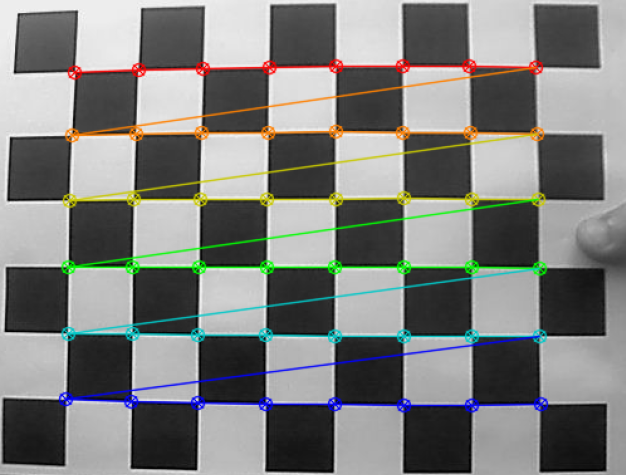
\includegraphics[width=4cm]{img1.png}
    \caption{3D points projected onto checkerboard's image}
    \label{fig:galaxy}
\end{figure}

\subsection{Finding camera matrix, K}

Now we could decompose homography matrix, $H$ to obtain K.

Writing $H$ in column form, we have $H = \begin{bmatrix} h_{1} & h_{2} & h_{3} \end{bmatrix}$. So,
\begin{center}
    \\$\begin{bmatrix} h_{1} & h_{2} & h_{3}\end{bmatrix} = K \begin{bmatrix} r_{1} & r_{2} & t\end{bmatrix}$\\ 
    $r_{1} = K^{-1} h_{1}$\\
    $r_{2} = K^{-1} h_{2}$
\end{center}

As $r_1$ and $r_2$ are orthonormal vectors, so they follow:
\begin{align*}
    \Vec{r_1}^T \Vec{r_2} &= 0\\
    \|\Vec{r_1}\| &= \|\Vec{r_2}\| = 1 
\end{align*}

Substituting value of $\Vec{r_1}$ and $\Vec{r_2}$ from above equations, we have:
\begin{align*}
    h_1^{T}K^{-T}K^{-1}h_2 &= 0\\
    h_1^{T}K^{-T}K^{-1}h_1 &= h_2^{T}K^{-T}K^{-1}h_2\\
    \text{Then taking RHS to LHS, we have:}\\
    h_1^{T}K^{-T}K^{-1}h_1 - h_2^{T}K^{-T}K^{-1}h_2 &= 0\\
\end{align*}
Let,  $B = K^{-T}K^{-1}$, which would be a symmetric matrix, so our pair of equations reduced to:\\
\begin{align*}
    h_1^{T}Bh_2 &= 0\\
    h_1^{T}Bh_1 - h_2^{T}Bh_2 &= 0\\
\end{align*}

Writing above equations in matrix form:
\begin{align*}
    V\Vec{b} &= \Vec{0}\\
    \text{where, V is given by:}\\
    V &= \begin{bmatrix}\Vec{v}_{12}^{T} \\ \Vec{v}_{11}^{T} - \Vec{v}_{22}^{T}\end{bmatrix}\\
\end{align*}
again, $\Vec{v}_{ij}$ is a column vector, composed of elements of $H$ matrix, given by:
\begin{align*}
    \Vec{v}_{ij} = \begin{bmatrix} h_{1i}h_{1j}\\ h_{1i}h_{2j} + h_{2i}h_{1j} \\ h_{3i}h_{1j} + h_{1i}h_{3j} \\ h_{2i}h_{2j} \\ h_{3i}h_{2j} + h_{2i}h_{3j} \\ h_{3i}h_{3j} \end{bmatrix}
\end{align*}
and, $\Vec{b} = [b_{11}, b_{12}, b_{13}, b_{22}, b_{23}, b_{33}]^T$  \\
As $\Vec{b}$ is a symmetric matrix, we only consider the 6 upper triangular elements. Now, we can solve the equation $V\Vec{b} &= \Vec{0}$, using SVD decomposition of $V$ to obtain $\Vec{b}$.\\
After reshaping $\Vec{b}$ into a $3\times3$ matrix, we could get original $B$. As $B$ is symmetric matrix, it cholesky decomposition would give $K$:
\begin{align*}
    AA^{T} &= choleskyDecomp(B)\\
    \text{As we assumed before, that } B = K^{-T}K^{-1}\text{, then A would be: }\\
    A &= K^{-T}\\
    \text{so, } K &= A^{-T}
\end{align*}

\subsection{Finding camera's Pose, R and T}

Now we know homography, $H$ and camera matrix, $K$. Next we want to find out the pose, $R$ and $t$ of camera. So, We have:
\begin{align*}
    H &= K \begin{bmatrix} r_1 & r_2 & t \end{bmatrix}\\
    K^{-1}H &= \begin{bmatrix} r_1 & r_2 & t \end{bmatrix}\\
\end{align*}
Let,  $K^{-1}H = \begin{bmatrix} h_1 & h_2 & h_3\end{bmatrix}$, then ideally we would have rotation matrix $M$ and translation vector $t$, given by: 
\begin{align*}
    M &= \begin{bmatrix} m_1 & m_2 & m_3\end{bmatrix}, \text{where, }\\
    m_1 &= \frac{h_1}{\|h_1\|_2}\\
    m_2 &= \frac{h_2}{\|h_1\|_2}\\
    m_3 &= m_1 \times m_2\\
    \text{and, }\\
    t &= \frac{h_3}{\|h_1\|}
\end{align*}

But for a matrix to be a rotation matrix, its column should be orthonormal and its determinant should be $1$. However there is no condition on a vector to be a translational vector. So we could accept $t$ as translation of checkerboard from camera. But we need to find a matrix, $R$ close to current matrix, $M$ and should also follows rotation matrix property, i.e. $R \in SO(3)$.\\
We could find such $R$, by solving:
\begin{align*}
    \underset{R \in SO(3)}{argmin}\|R - M\|_{F}^2
\end{align*}

The solution is given by SVD of matrix, $M$ as: 
\begin{align*}
    USV^{T} &= SVD(M)\\
    \text{Then matrix R would be:}\\
    R &= U\begin{bmatrix}1 & 0 & 0\\ 0 & 1 & 0\\ 0 & 0 & det(UV^{T})\end{bmatrix}V^{T}
\end{align*}

By approximating S matrix to the above form, we are ensuring $R \in SO(3)$, i.e., diagonal matrix is ensuring that $det(R) = 1$, while product of $U$ and $V^{T}$, is ensuring that resulting matrix has orthogonal columns.  

\begin{thebibliography}{9}
    \bibitem{latex} An Invitation to 3-D Vision: From Images to Geometric Models, Jana Košecká et al.
    \bibitem{latex} Lecture: Cyrill Stachniss, Photogrammetry I, YouTube.
    \bibitem{latex} Lecture: Kostas Daniilidis, CIS 390, Robotics: Planning and Perception.
\end{thebibliography}

\end{document}
